\documentclass[final]{beamer}

\usepackage[scale=1.24]{beamerposter} % Use the beamerposter package for laying out the poster
\usetheme{confposter} % Use the confposter theme supplied with this template

\setbeamercolor{block title}{fg=ngreen,bg=white} % Colors of the block titles
\setbeamercolor{block body}{fg=black,bg=white} % Colors of the body of blocks
\setbeamercolor{block alerted title}{fg=white,bg=dblue!70} % Colors of the highlighted block titles
\setbeamercolor{block alerted body}{fg=black,bg=dblue!10} % Colors of the body of highlighted blocks

%-----------------------------------------------------------
% Define the column widths and overall poster size
% To set effective sepwid, onecolwid and twocolwid values, first choose how many columns you want and how much separation you want between columns
% In this template, the separation width chosen is 0.024 of the paper width and a 4-column layout
% onecolwid should therefore be (1-(# of columns+1)*sepwid)/# of columns e.g. (1-(4+1)*0.024)/4 = 0.22
% Set twocolwid to be (2*onecolwid)+sepwid = 0.464
% Set threecolwid to be (3*onecolwid)+2*sepwid = 0.708

\newlength{\sepwid}
\newlength{\onecolwid}
\newlength{\twocolwid}
\newlength{\threecolwid}
% \setlength{\paperwidth}{91cm} % A0 width: 46.8in
% \setlength{\paperheight}{61cm} % A0 height: 33.1in

\setlength{\paperwidth}{48in} % A0 width: 46.8in
\setlength{\paperheight}{36in} % A0 height: 33.1in

% Posters should be of size 61 cm x 91 cm in portrait orientation or 90 x 122 cm in landscape orientation.

\setlength{\sepwid}{0.024\paperwidth} % Separation width (white space) between columns
\setlength{\onecolwid}{0.22\paperwidth} % Width of one column
\setlength{\twocolwid}{0.464\paperwidth} % Width of two columns
\setlength{\threecolwid}{0.708\paperwidth} % Width of three columns
\setlength{\topmargin}{-0.5in} % Reduce the top margin size
%-----------------------------------------------------------

\usepackage{graphicx}  % Required for including images
\usepackage{booktabs} % Top and bottom rules for tables

\title{COMS W4995 Final Report: Automatic Data Augmentation Policy Selection} % Poster title
\author{Jonathan D. Armstrong, Jesse Galef, and Kyle Matoba} % Author(s)
\institute{Computer Science Department, Columbia University} % Institution(s)

%----------------------------------------------------------------------------------------

\begin{document}

\addtobeamertemplate{block end}{}{\vspace*{2ex}} % White space under blocks
\addtobeamertemplate{block alerted end}{}{\vspace*{2ex}} % White space under highlighted (alert) blocks

\setlength{\belowcaptionskip}{2ex} % White space under figures
\setlength\belowdisplayshortskip{2ex} % White space under equations

\begin{frame}[t] % The whole poster is enclosed in one beamer frame
\begin{columns}[t] % The whole poster consists of three major columns, the second of which is split into two columns twice - the [t] option aligns each column's content to the top

\begin{column}{\sepwid}\end{column} % Empty spacer column
\begin{column}{\onecolwid} % The first column

\begin{alertblock}{Objectives}
Approach or improve upon state of the arts results in image classification on the CIFAR-10 dataset (\cite{Krizhevsky2009}) through better, automatically chosen, data augmentation methods. 

\begin{itemize}
\item \cite{Cubuk2018}
\end{itemize}

\end{alertblock}

%----------------------------------------------------------------------------------------
%	INTRODUCTION
%----------------------------------------------------------------------------------------

\begin{block}{Introduction}

Data augmentation has proven essential for obtaining state of the art performance on image classification. For example, 

\begin{figure}
\centering
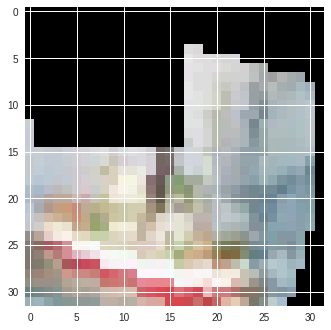
\includegraphics[width=0.70\textwidth]{ship.png}
\caption{An augmented CIFAR 10 picture labelled as a ship}
\end{figure}

\end{block}
\end{column} % End of the first column

\begin{column}{\sepwid}\end{column} % Empty spacer column
\begin{column}{\twocolwid} % Begin a column which is two columns wide (column 2)
\begin{columns}[t,totalwidth=\twocolwid] % Split up the two columns wide column

\begin{column}{\onecolwid}\vspace{-.6in} % The first column within column 2 (column 2.1)

% MATERIALS

\begin{block}{Wide ResNet}
\cite{Zagoruyko2016}
\begin{itemize}
\item Duis porta consequat lorem
\item Eu facilisis est tempus quis
\end{itemize}

\end{block}

%----------------------------------------------------------------------------------------

\end{column} % End of column 2.1

\begin{column}{\onecolwid}\vspace{-.6in} % The second column within column 2 (column 2.2)

%----------------------------------------------------------------------------------------
%	METHODS
%----------------------------------------------------------------------------------------

\begin{block}{Methods}

Lorem ipsum dolor \textbf{sit amet}, 

\end{block}
\end{column} % End of column 2.2
\end{columns} % End of the split of column 2 - any content after this will now take up 2 columns width

%	IMPORTANT RESULT

\begin{alertblock}{Hardware Accelerators}

\end{alertblock} 

%----------------------------------------------------------------------------------------

\begin{columns}[t,totalwidth=\twocolwid] % Split up the two columns wide column again
\begin{column}{\onecolwid} % The first column within column 2 (column 2.1)

%----------------------------------------------------------------------------------------
%	MATHEMATICAL SECTION
%----------------------------------------------------------------------------------------

\begin{block}{Mathematical Section}

Nam quis odio enim, in molestie libero. Vivamus cursus mi at nulla elementum sollicitudin. Nam quis odio enim, in molestie libero. Vivamus cursus mi at nulla elementum sollicitudin.
  
\begin{equation}
E = mc^{2}
\label{eqn:Einstein}
\end{equation}

Nam quis odio enim, in molestie libero. Vivamus cursus mi at nulla elementum sollicitudin. Nam quis odio enim, in molestie libero. Vivamus cursus mi at nulla elementum sollicitudin.

\begin{equation}
\cos^3 \theta =\frac{1}{4}\cos\theta+\frac{3}{4}\cos 3\theta
\label{eq:refname}
\end{equation}

Nam quis odio enim, in molestie libero. Vivamus cursus mi at nulla elementum sollicitudin. Nam quis odio enim, in molestie libero. Vivamus cursus mi at nulla elementum sollicitudin.

\begin{equation}
\kappa =\frac{\xi}{E_{\mathrm{max}}} %\mathbb{ZNR}
\end{equation}

\end{block}

%----------------------------------------------------------------------------------------

\end{column} % End of column 2.1

\begin{column}{\onecolwid} % The second column within column 2 (column 2.2)

%----------------------------------------------------------------------------------------
%	RESULTS
%----------------------------------------------------------------------------------------

\begin{block}{Results}

\begin{figure}
\includegraphics[width=0.8\linewidth]{placeholder.jpg}
\caption{Figure caption}
\end{figure}

Nunc tempus venenatis facilisis. Curabitur suscipit consequat eros non porttitor. Sed a massa dolor, id ornare enim:

\begin{table}
\vspace{2ex}
\begin{tabular}{l l l}
\toprule
\textbf{Treatments} & \textbf{Response 1} & \textbf{Response 2}\\
\midrule
Treatment 1 & 0.0003262 & 0.562 \\
Treatment 2 & 0.0015681 & 0.910 \\
Treatment 3 & 0.0009271 & 0.296 \\
\bottomrule
\end{tabular}
\caption{Table caption}
\end{table}

\end{block}

%----------------------------------------------------------------------------------------

\end{column} % End of column 2.2

\end{columns} % End of the split of column 2

\end{column} % End of the second column

\begin{column}{\sepwid}\end{column} % Empty spacer column

\begin{column}{\onecolwid} % The third column

\begin{block}{An interesting finding about CIFAR 10 data}

\texttt{import keras} \\
\texttt{import matplotlib.pyplot as plt} \\

\texttt{labels = ['plane', 'car', 'bird', 'cat', 'deer', 'dog', 'frog', 'horse', 'ship', 'truck']} \\
\texttt{\_, (x, y) = keras.datasets.cifar10.load\_data()} \\
\texttt{plt.imshow(x[2405, :, :, :])} \\
\texttt{plt.title(labels[y[2405, 0]])}

\begin{figure}
\centering
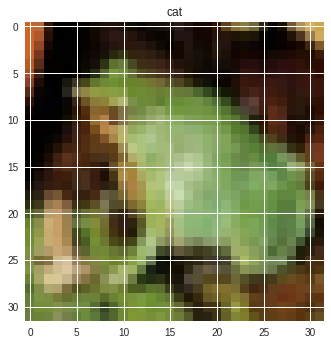
\includegraphics[width=0.70\linewidth]{catfrog.png}
\end{figure}

Fundamental upper bound on achievable accuracy?
\end{block}

% CONCLUSION

\begin{block}{Conclusion}
We have demonstrated that very simple policy searches suffice for obtaining nearly optimal performance-enhancing image augmentation. Together with a relatively lightweight Wide ResNet fit upon a free TPU, we are able to present an at-or-near state of the art CIFAR-10 image classifier that is achievable to 

\end{block}

% ADDITIONAL INFORMATION
% 
% \begin{block}{Additional Information}
% 
% Maecenas ultricies feugiat velit non mattis. Fusce tempus arcu id ligula varius dictum. 
% \begin{itemize}
% \item Curabitur pellentesque dignissim
% \end{itemize}
% 
% \end{block}

\begin{block}{References}

% \nocite{*} % Insert publications even if they are not cited in the poster
% \small{\bibliographystyle{unsrt}
% \bibliography{sample}\vspace{0.75in}}

{\small
\bibliographystyle{ieee}
\bibliography{../biblio}
}
\end{block}

% ACKNOWLEDGEMENTS
\setbeamercolor{block title}{fg=red,bg=white} % Change the block title color
\begin{block}{Acknowledgements}
Many thanks to Professor Drori for his help and encouragement. \\
\end{block}

% CONTACT INFORMATION
\setbeamercolor{block alerted title}{fg=black,bg=norange} % Change the alert block title colors
\setbeamercolor{block alerted body}{fg=black,bg=white} % Change the alert block body colors

\begin{alertblock}{Contact Information}
\begin{itemize}
\item Jonathan: \href{mailto:jda2160@columbia.edu}{jda2160@columbia.edu}
\item Jesse: \href{mailto:jbg2160@columbia.edu}{jbg2160@columbia.edu}
\item Kyle: \href{mailto:km3227@columbia.edu}{km3227@columbia.edu}
\end{itemize}

\end{alertblock}

\begin{center}

\includegraphics[width=0.8\linewidth]{logo.jpg} % & \hfill & 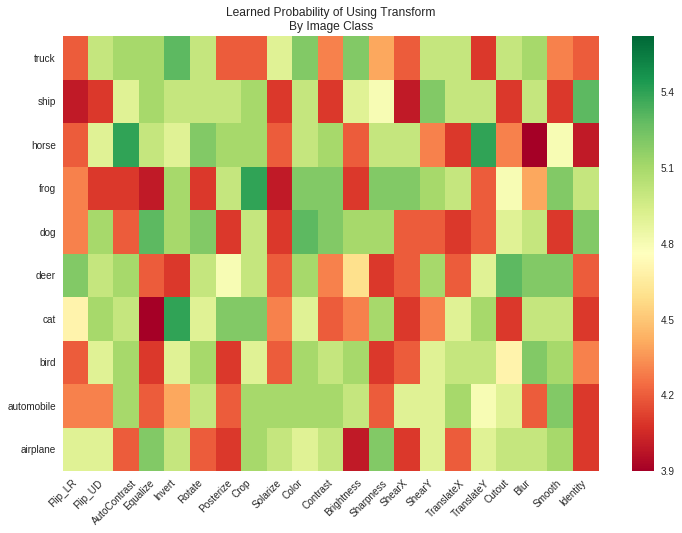
\includegraphics[width=0.4\linewidth]{logo.png}
\end{center}

\end{column} % End of the third column
\end{columns} % End of all the columns in the poster
\end{frame} % End of the enclosing frame
\end{document}
